\chapter{Theoretische Grundlagen} \label{chap:theoretische_grundlagen}  % Theorie
Zu Beginn dieser Studienarbeit werden die theoretischen Grundlagen erläutert, die für das Verständnis der späteren Kapitel notwendig sind. Dazu gehören die Funktionsweise von Machine Learning und Computer Vision, sowie die Grundlagen einer API.
Wie bereits im Ersten Kapitel (siehe Kapitel \ref{chap:problemstellung_und_ziel_dieser_arbeit}) beschrieben, baut diese Studienarbeit auf der Arbeit des letzten Semesters auf. 
Die theoretischen Grundlagen für Machine Learning und Computer Vision werden hier nur kurz erläutert, da sie bereits im letzten Semester ausführlich behandelt wurden.

Die Funktionsweise einer API wird in diesem Kapitel genauer erläutert, da sie eine zentrale Rolle in dieser Studienarbeit spielt. Mithilfe einer Web-API werden die Daten
des Python programmes an die entwickelte Webanwendung übertragen.

\section{Machine Learning und Klassifikationsprobleme} \label{sec:ml_cv}  % Theorie
Grundlegend, bevor die Datensätze in Form von Bildern durch Convoliutional Neural Networks \ac{CNN} analysiert werden können, müssen die Daten verarbeitet werden.

Bildverarbeitung beschäftigt sich mit der Manipulation und Analyse digitaler Bilder durch Algorithmen und bildet die Grundlage für komplexere Verfahren. 
Ein digitales Bild wird als mehrdimensionale Matrix gespeichert, wobei farbige Bilder als dreidimensionale Tensoren 
dargestellt werden, deren Dimensionen Höhe, Breite und Farbkanäle repräsentieren. 
Diese Repräsentation ermöglicht die Anwendung verschiedener Transformationen wie Filterung, Kontrastverbesserung oder geometrische Verzerrungen, die 
entweder zur Bildverbesserung oder als Vorverarbeitungsschritte für nachfolgende Analysen durch fortschrittlichere Techniken wie Machine Learning und Computer Vision dienen \cite{finbridgede_computer_2022}.

Convolutional Neural Networks \ac{CNN} sind spezialisierte Deep Learning Modelle, die für die Verarbeitung von Bilddaten optimiert sind. Sie bilden die Grundlage für zahlreiche moderne Computer Vision Anwendungen, wie Gesichtserkennung und autonome Fahrzeuge. 
Die Architektur eines CNN nutzt die räumliche Struktur von Bildern effizient, um visuelle Muster zu erkennen und zu klassifizieren.
Ein CNN besteht hauptsächlich aus Faltungsschichten und Linearen Ebenen (siehe \autoref{fig:system_overview}). 
Die Convolutional Layers verwenden kleine Filtermatrizen (Kernel), die über das Bild gleiten und visuelle Merkmale wie Kanten und Texturen erkennen. 
Diese Filter werden während des Trainings optimiert, um die relevantesten Merkmale zu extrahieren \cite{finbridgede_computer_2022} \cite{intel_convolutional_nodate}.

\begin{figure}[h]
    \centering
    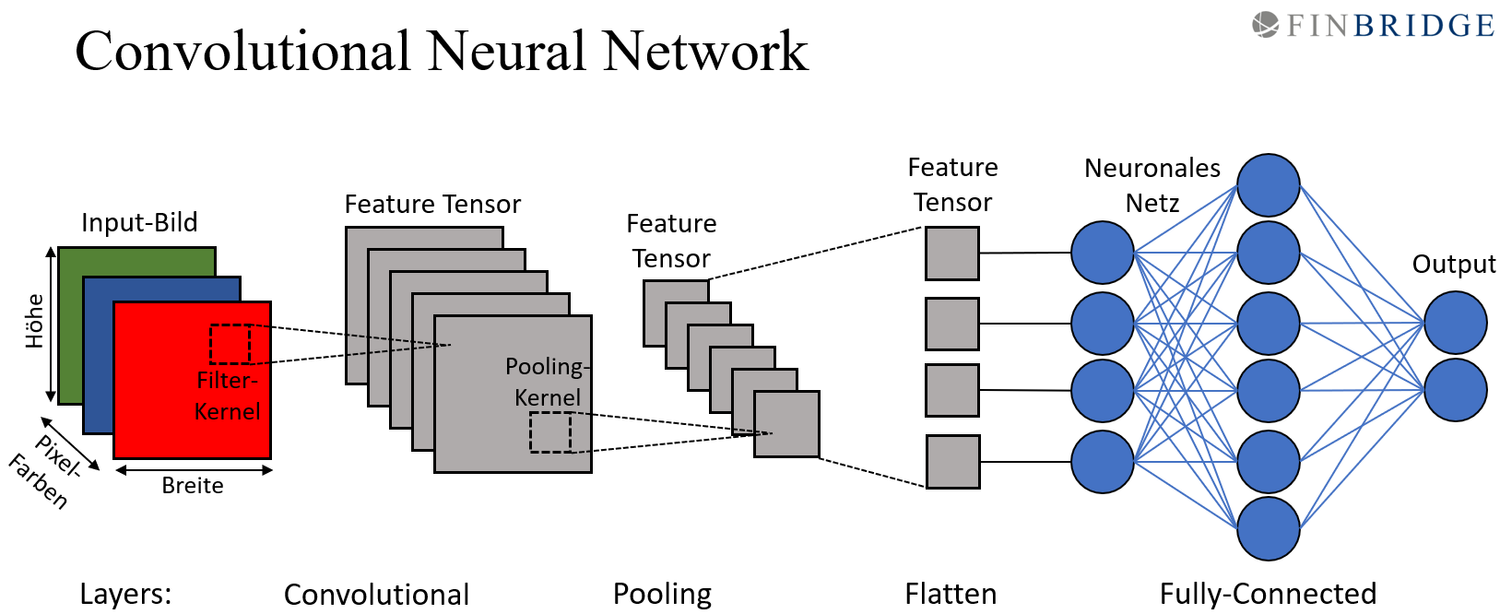
\includegraphics[width=1\textwidth]{CNN.png}
    \caption{Aufbau eines Convolutional Neural Networks \cite{finbridgede_computer_2022}.}
    \label{fig:system_overview}
\end{figure}

Die Fully-Connected Layers am Ende des Netzwerks (siehe \autoref{fig:system_overview}) wandeln die extrahierten Merkmale in eine endgültige Klassifikation oder Vorhersage um. Diese Schichten sind ähnlich wie traditionelle neuronale Netzwerke aufgebaut, wobei jedes Neuron mit allen Neuronen der vorherigen Schicht verbunden ist.

Die wichtigsten Lernansätze im maschinellen Lernen sind überwachtes, unüberwachtes und verstärkendes Lernen. In dieser Arbeit wird überwachtes Lernen genutzt, bei dem ein Algorithmus mit gelabelten Daten trainiert wird, um aus diesen Beispielen zu lernen und Vorhersagen zu treffen.

Beim überwachten Lernen gibt es zwei Hauptmodelle: Klassifikation und Regression. Regression beschreibt kontinuierliche Zusammenhänge zwischen Eingangs- und Ausgangsdaten \cite{noauthor_machine_nodate-1}. Klassifikation teilt Daten in diskrete Gruppen ein. Es sollen keine Kontinuierlichen werte nachgebildet werden. Am Ende des Netzwerks wird mithifge einer $argmax()$ Funktiion eine Klasse fest zugeordnet \cite[S. 450]{suse_bildverarbeitung_2014}. Die binäre Klassifikation, welche in dieser Arbeit angewandt wird ist eine spezielle Form der Klassifikation, bei der nur zwei Klassen unterschieden werden.

Es gibt verschiedene CNN-Architekturen wie ResNet und MobileNet, die für spezifische Aufgaben besonders gut geeignet sind. Oft werden vortrainierte Modelle verwendet und für spezifische Anwendungsfälle feinabgestimmt, eine Technik bekannt als Transfer Learning, welche auf dem überwachten Lernen basiert. \cite{finbridgede_computer_2022}.

\section{Die Funktionsweise einer API} \label{sec:api}  % Theorie

APIs stellen das Herzstück moderner Softwareentwicklung dar und ermöglichen es Programmen, miteinander zu kommunizieren und Daten auszutauschen. Dieser Datenaustausch ist wesentlich für vielfältige Anwendungen, wie etwa das Abrufen von Wetterdaten oder das Interagieren mit sozialen Netzwerken. In der Python Entwicklungsumgebung machen Bibliotheken wie requests oder http.client den Einstieg in die API-Entwicklung besonders zugänglich \cite{software_mittelstand_erste_nodate}. Die in dieser Studienarbeit verwendete FLASK Bibliothek ermöglicht es, eine komplextere API zu erstellen, die Daten aus dem Python Programm an die Webanwendung überträgt.

Anwendungsprogrammierschnittstellen \ac{API} sind Software-Vermittler (\autoref{fig:api_design}) ihre Aufgabe besteht darin, Anwendungen die Kommunikation untereinander zu ermöglichen. 
Diese subtilen Vermittler sind allgegenwärtig im täglichen Leben, ob bewusst wahrgenommen oder nicht \cite{pykes_programmieren_nodate}.

\begin{figure}[h]
    \centering
    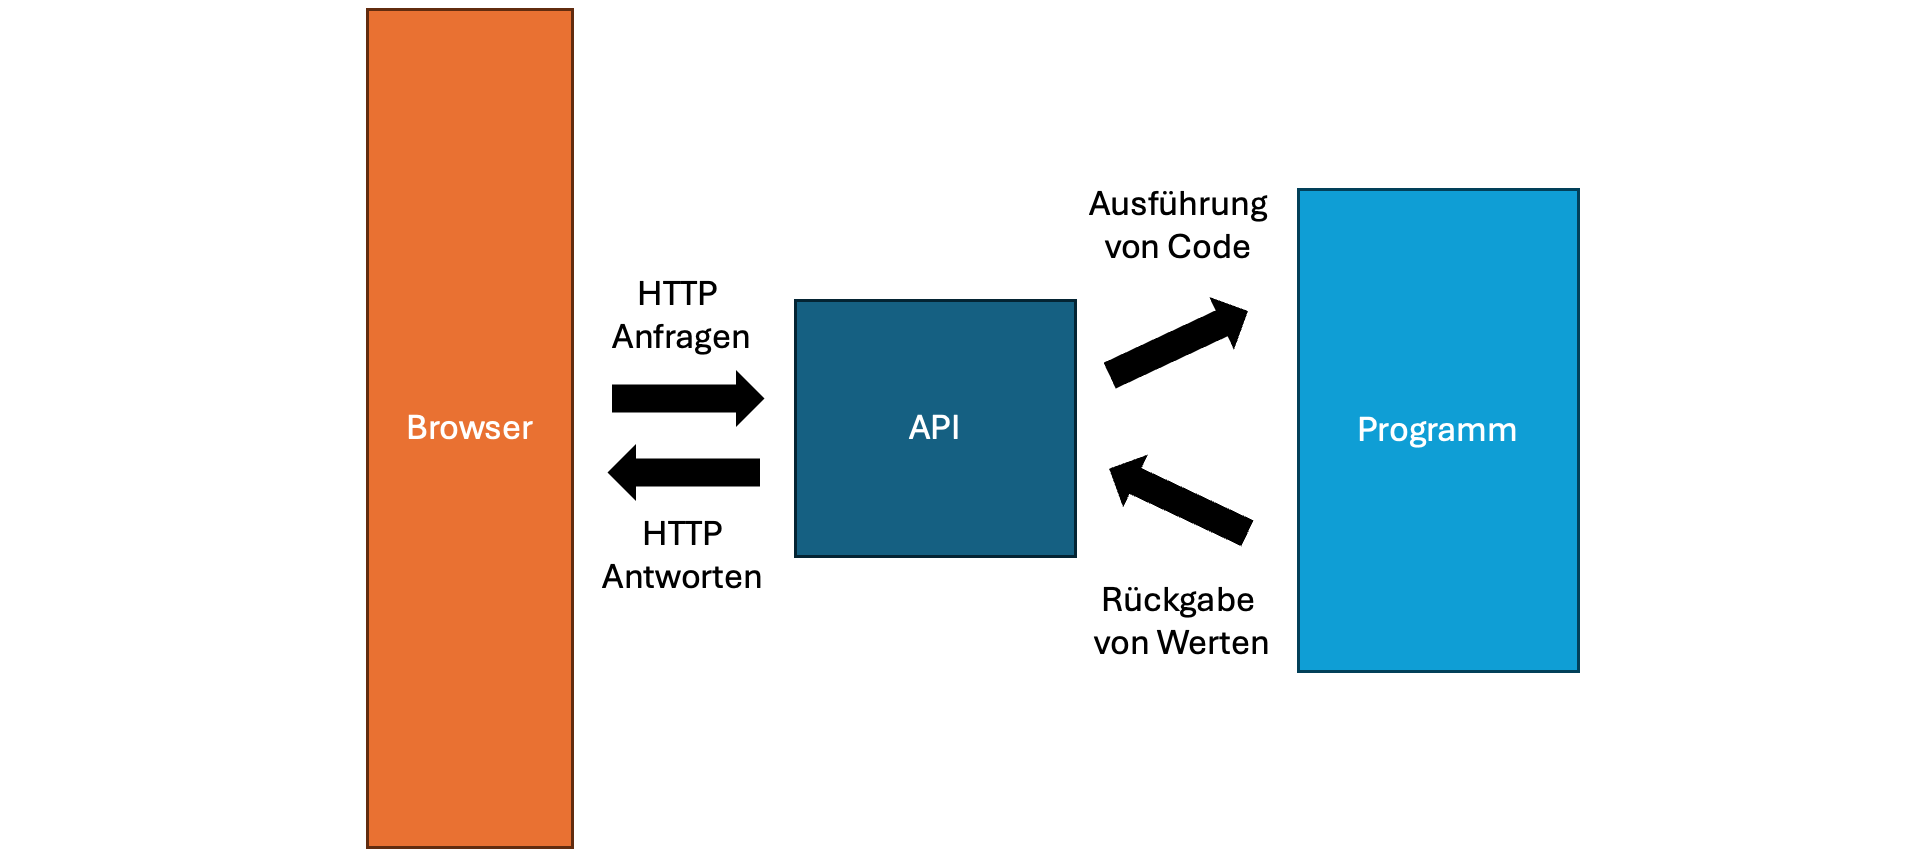
\includegraphics[width=1\textwidth]{API.png}
    \caption{Schematischer Aufbau der API Kommunikation}
    \label{fig:api_design}
\end{figure}

Im Kontext von Webanwendungen bieten \ac{API}s den Zugriff auf Daten und Funktionalitäten von Drittanbietern. 
Dies ermöglicht es Entwicklern, ihre Anwendungen um Funktionen wie Wetterinformationen, Sportergebnisse, Filmlisten, Tweets, Suchmaschinenergebnisse und Bildverarbeitung zu erweitern. 
Die Eigenentwicklung solcher Funktionen würde erhebliche Ressourcen beanspruchen, während die Nutzung von APIs eine schnelle und effiziente Integration ermöglicht\cite{digital_ocean_llc_erste_nodate}.

\subsection{Anfragearten einer API} \label{subsec:anfragearten_einer_api}  % Theorie

Die Grundbausteine einer \Ac{API} sind Anfragen (Requests) und Antworten (Responses). Diese basieren oft auf dem \ac{HTTP}-Protokoll, das die Grundlage des Internets bildet \cite{software_mittelstand_erste_nodate}. 
\ac{HTTP}-Anfragen sind die Art und Weise, wie das Web funktioniert. Jedes Mal, wenn man zu einer Webseite navigiert, stellt der Browser mehrere Anfragen an den Server der Webseite. Der Server antwortet dann mit allen Daten, die für die Darstellung der Seite erforderlich sind, woraufhin der Browser die Seite darstellt \cite{digital_ocean_llc_erste_nodate}.

Der generische Prozess der \Ac{API}-Kommunikation lässt sich wie folgt beschreiben: Ein Client, in dieser Studienarbeit der Browser, sendet Daten an eine Uniform Resource Locator \ac{URL}. Der Server unter dieser \ac{URL} liest die Daten, entscheidet, was damit zu tun ist. Intern wird das passende Python Skript ausgeführt und gibt eine Antwort an den Client zurück. Schließlich verarbeitet der Client die empfangenen Daten entsprechend seiner Programmlogik \cite{digital_ocean_llc_erste_nodate}.

Ein wesentlicher Teil der Anfrage ist die Hypertext Transfer Protocol \ac{HTTP}-Methode. Einige der gebräuchlichsten Methoden sind \cite{rodriguez_rest_2016}:
\begin{itemize}
    \item \textbf{GET} Dient dem Abrufen von Daten, ohne Änderungen auf dem Server vorzunehmen
    \item \textbf{POST} Wird verwendet, um neue Daten an den Server zu senden
    \item \textbf{PUT} Aktualisiert vorhandene Daten auf dem Server
    \item \textbf{DELETE} Entfernt Daten vom Server
\end{itemize}

Diese Methoden bilden die Grundlage des Representational State Transfer \ac{REST}ful API-Designs, das in modernen Webanwendungen weit verbreitet ist \cite{rodriguez_rest_2016}.

\subsection{FLASK} \label{subsec:flask}  % Theorie

Für diese Studienarbeit ist keine Umfängliche WEB-\ac{API} notwendig. Es soll lediglich eine einzige \ac{HTML} Datei von der Python Anwendung an den Browser übertragen werden. Es ist für diese Anforderung kein Größeres Framework wie Beispielsweise Django notwendig. FLASK ist ein Mikroframework für Python, das sich auf einfache und schnelle Entwicklung konzentriert. Es ist besonders gut geeignet für kleine bis mittelgroße Projekte, bei denen die Verwendung eines größeren Frameworks übertrieben wäre. FLASK bietet eine Vielzahl von Erweiterungen, die die Entwicklung von Webanwendungen erleichtern. Es ist einfach zu erlernen und bietet eine Vielzahl von Funktionen, die für die Entwicklung von Webanwendungen erforderlich sind.

\begin{figure}[h]
    \centering
    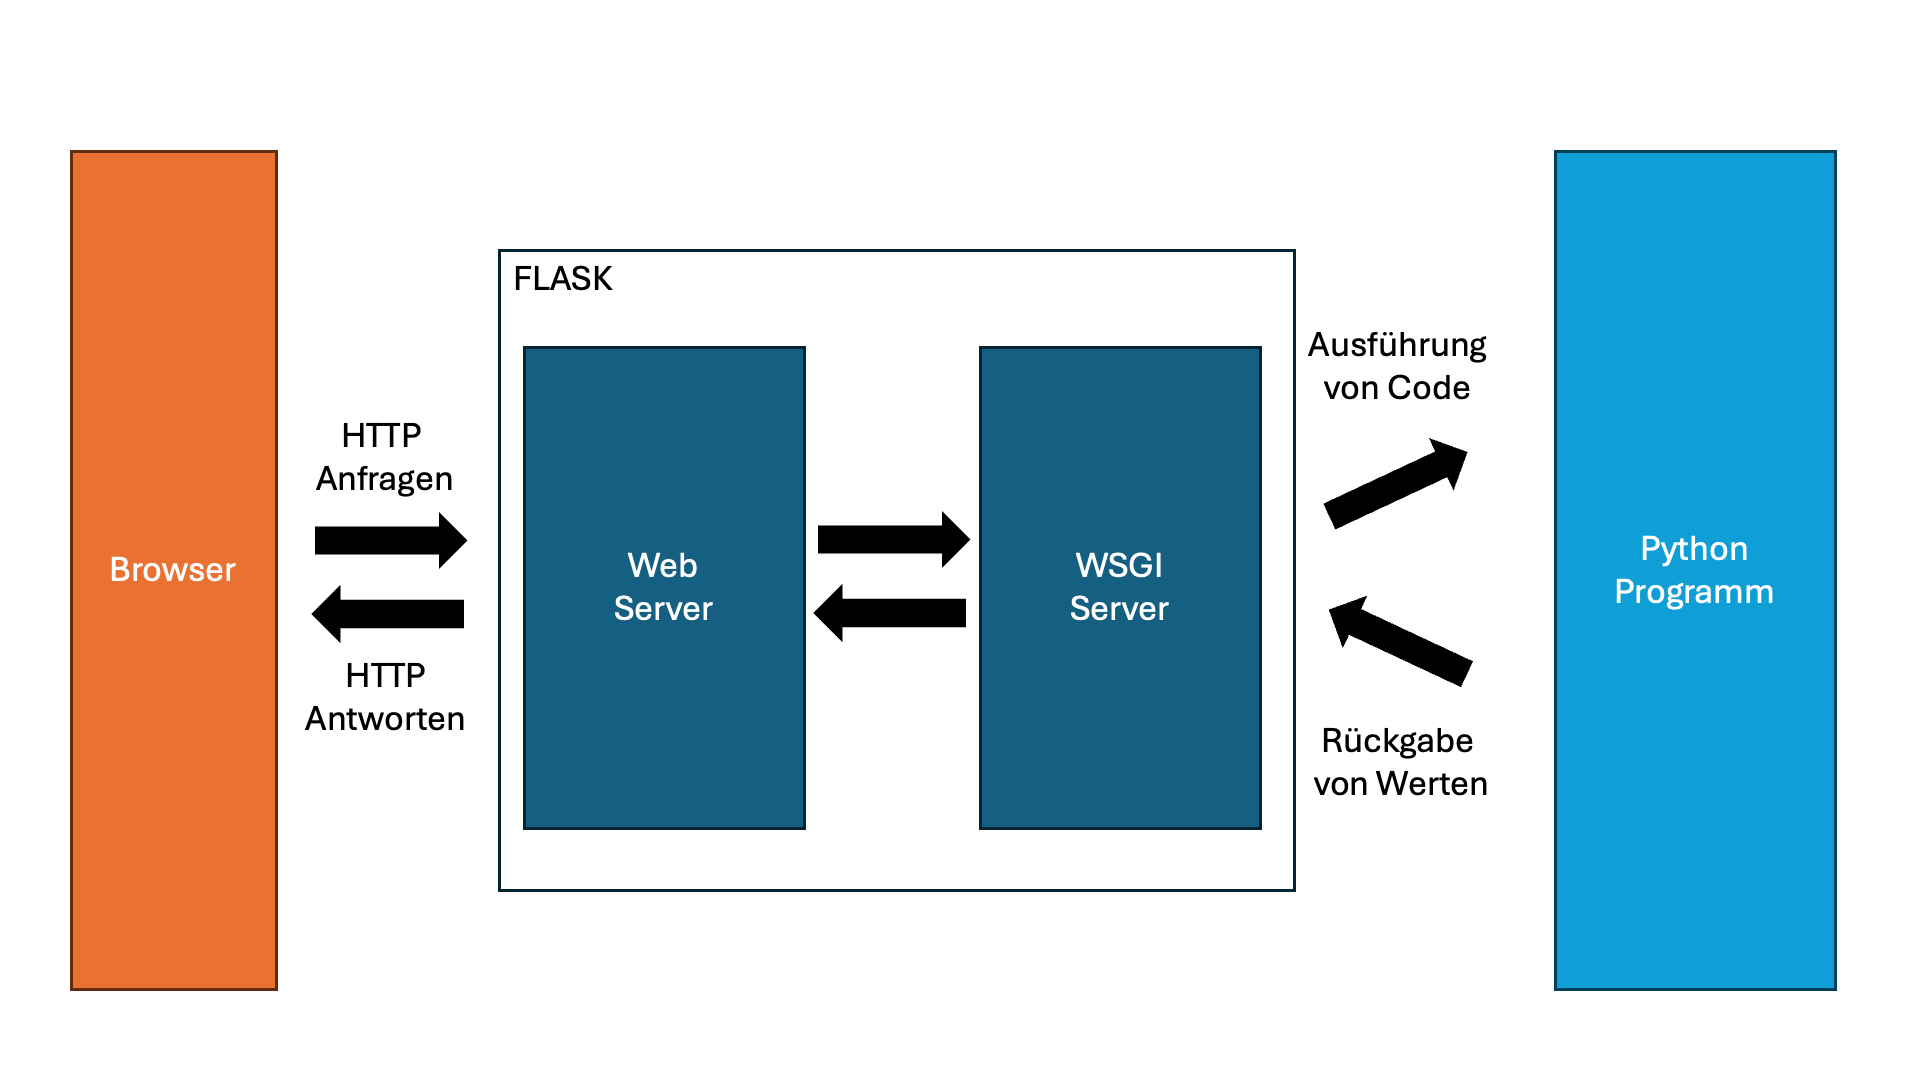
\includegraphics[width=1\textwidth]{FLASK.png}
    \caption{Erweiterung der API Darstellung auf Basis von FLASK}
    \label{fig:flask}
\end{figure}

FLASK Nutzt die \ac{WSGI} Schnittstelle von Python \cite{flask_welcome_nodate} und  \autoref{fig:flask} und Stellt in Verbindung mit der in dieser Studienarbeit Verwendeten Waitress Bibliothek den Webserver zur Verfügung.

Eine Besondere Anforderung der im Folgenden vorgestellten Webanwendung liegt in der Übertragung der neu erstellten Fotos von der Kamera des FESTO \ac{cp-lab} an die 
Webanwendung. Um eine einfachere Benutzbarkeit zu gewährleisten soll der Browser nicht jedes mal neu geladen werden müssen, wenn ein Foto geschossen und klassifiziert wird.

Dies geschieht durch die Verwendung von Websockets. Websockets sind eine Technologie, die es ermöglicht, eine bidirektionale Verbindung zwischen einem Client und einem Server herzustellen.
FLASK SocketIO ist eine Erweiterung für FLASK, die die Verwendung von Websockets in FLASK Anwendungen ermöglicht und wird in dieser Studienarbeit verwendet, um die Übertragung der Fotos zu realisieren. 
Auf der gegenseite im HTML Code wird die Bibliothek SocketIO.js verwendet. 
Diese Basiert auf der Programmiersprache JavaScript und ermöglicht die Kommunikation zwischen dem Browser und dem Server.

Im Folgenden wird die neue Softwarearchitektur vorgestellt und auch die Implementierung der Webanwendung erläutert.